\section{Descrição do Conjunto de Dados}

A campanha de campo foi conduzida em um ambiente de água doce na região amazônica (Itacoatiara, AM, Brasil), com pontos de amostragem georreferenciados distribuídos para capturar gradientes espaciais locais. O conjunto de dados inclui a posição em UTM 21S e variáveis físico-químicas usadas como entradas e saídas do modelo, e está publicamente disponível no Mendeley Data \cite{assuncao2026dataset}. A cobertura espacial da campanha é mostrada na Fig.~\ref{fig:dataset_map}, e as estatísticas descritivas dos alvos de predição são reportadas na Tabela~\ref{tab:dataset_stats}.

A coleta de dados seguiu um desenho espacialmente distribuído para representar diferentes microzonas do lago, em vez de amostrar repetidamente uma única coordenada, apoiando a interpretação espacial e o suporte à decisão local (mapas de interpolação e índices compostos de triagem). As medições foram consolidadas em uma estrutura tabular adequada à inferência orientada à borda e ao treinamento reprodutível.

\subsection{Variáveis e Aquisição}
Os atributos de entrada foram $x$, $y$, temperatura (TEMP), cor aparente em escala âmbar (COR\_A) e índice visual de cor (COR\_V). As variáveis-alvo foram pH, oxigênio dissolvido (OD) e turbidez (TURB). \rev{O conjunto de dados original de campo compreende 60 amostras georreferenciadas.} O desenho amostral priorizou a representatividade espacial em detrimento da repetição temporal densa, de forma consistente com o objetivo de gerar superfícies espaciais interpretáveis.

\rev{A Tabela~\ref{tab:corr_analysis} reporta a correlação de Pearson entre cada atributo de entrada e cada alvo no conjunto original de 60 amostras. As coordenadas espaciais e os índices de cor estão fortemente associados ao pH (\mbox{$r=-0,85$} para $y$; \mbox{$r=-0,79$} para COR\_A) e à turbidez (\mbox{$r=0,69$} e \mbox{$r=0,68$}, respectivamente), indicando gradientes espaciais e ópticos exploráveis. Em contraste, o OD é fracamente correlacionado com todas as entradas disponíveis (\mbox{$|r| \leq 0,24$}), o que antecipa a maior dificuldade de predição desse alvo com o conjunto de atributos atual.}

\begin{table}[t]
\caption{\rev{Correlação de Pearson entre atributos de entrada e alvos (conjunto original, $n=60$).}}
\label{tab:corr_analysis}
\centering
\footnotesize
\setlength{\tabcolsep}{6pt}
\rowcolors{2}{yellow!30}{yellow!30}
\begin{tabular}{lccc}
\toprule
Atributo & pH & OD & TURB \\
\midrule
$x$ & $0.75$ & $-0.23$ & $-0.67$ \\
$y$ & $-0.85$ & $0.18$ & $0.69$ \\
TEMP & $-0.56$ & $0.24$ & $0.33$ \\
COR\_A & $-0.79$ & $0.05$ & $0.68$ \\
COR\_V & $-0.46$ & $0.08$ & $0.50$ \\
\bottomrule
\end{tabular}
\end{table}

\begin{figure}[t]
\centering
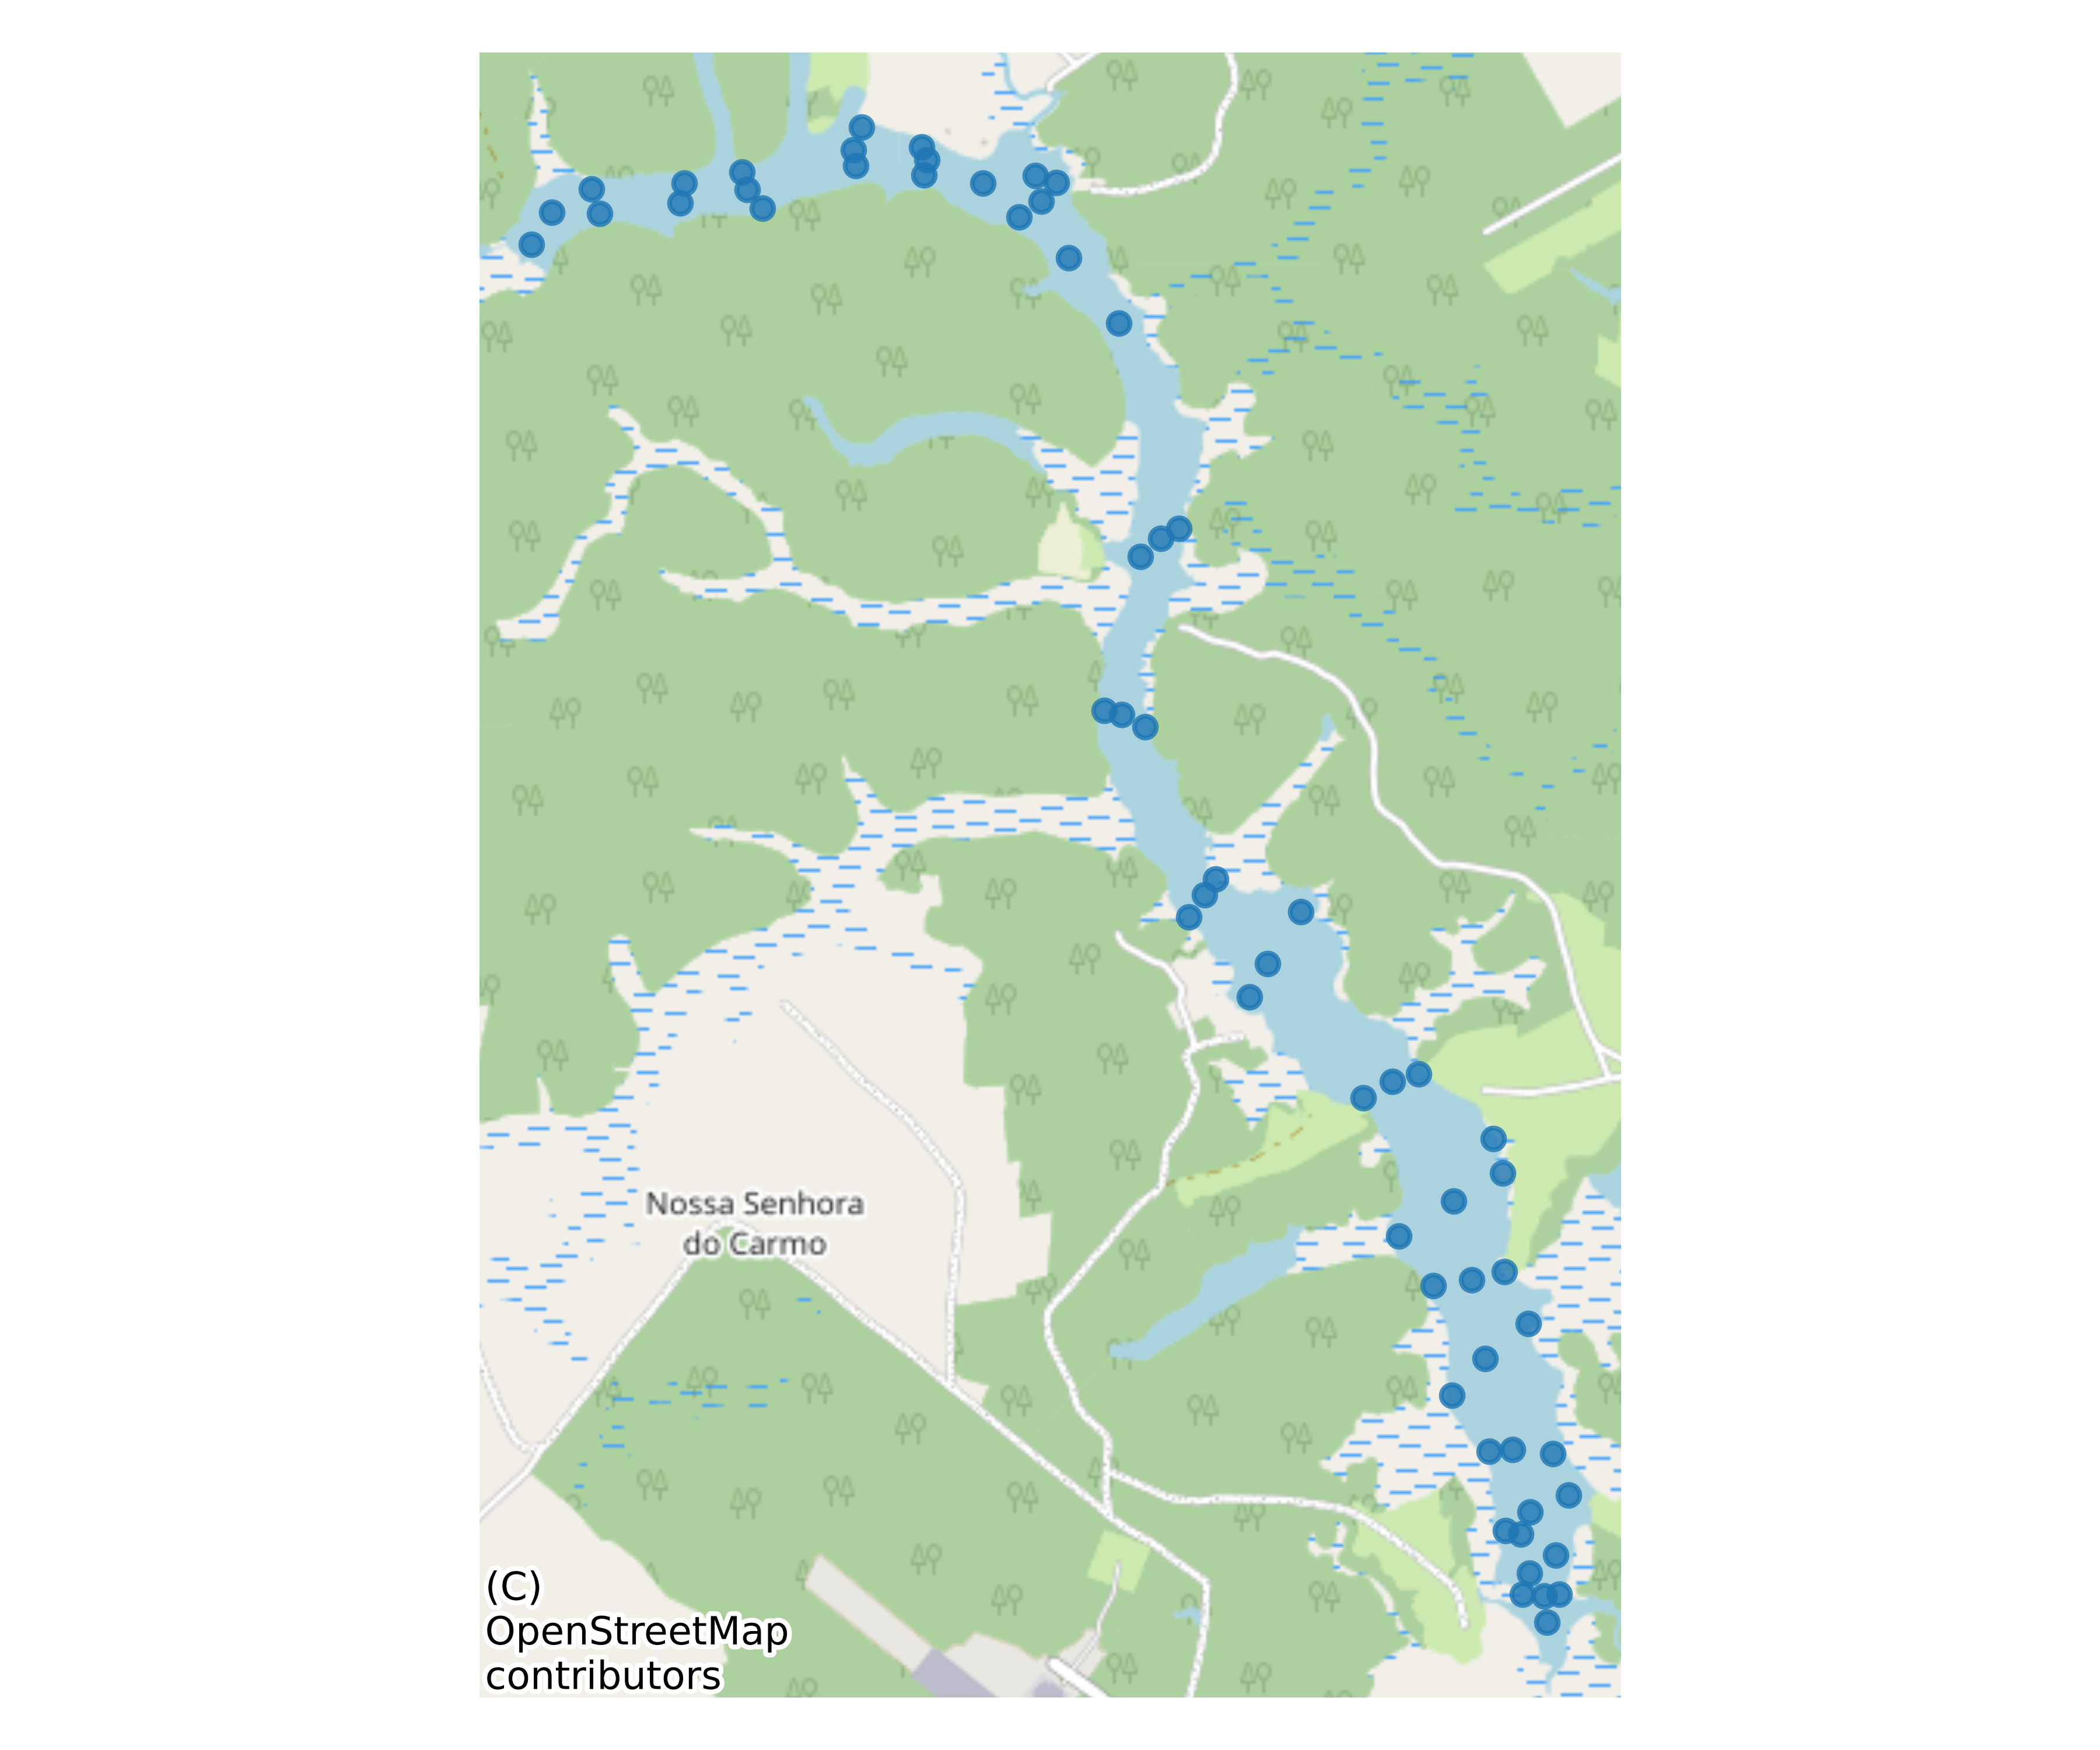
\includegraphics[width=0.64\linewidth]{map_points_osm_21S.png}
\caption{Localizações de amostragem sobre mapa-base OpenStreetMap (UTM 21S).}
\label{fig:dataset_map}
\end{figure}

\begin{table}[t]
\caption{Estatísticas descritivas dos alvos no conjunto de dados original de campo.}
\label{tab:dataset_stats}
\centering
\begin{tabular}{lcccc}
\toprule
Variável & Média & Desvio & Mín & Máx \\
\midrule
pH & 5.73 & 0.31 & 5.15 & 6.50 \\
OD (mg/L) & 1.86 & 0.32 & 1.26 & 2.52 \\
Turbidez (NTU) & 2.77 & 1.37 & 0.06 & 6.18 \\
\bottomrule
\end{tabular}
\end{table}

\subsection{Aumento de Dados}
Como o conjunto de dados original é pequeno \rev{($n=60$)}, aplicou-se aumento sintético com fator $\times 10$ usando perturbação gaussiana leve (\mbox{$\sigma=0,01$}) no espaço normalizado\rev{, resultando em 600 amostras de suporte ao treinamento}. Essa estratégia foi usada para estabilizar o treinamento e reduzir a sensibilidade à partição, preservando as distribuições marginais e a plausibilidade física. O conjunto aumentado é usado apenas como suporte ao treinamento e não representa medições de campo adicionais. \rev{A perturbação gaussiana foi adotada por sua transparência e baixo risco de distorção neste regime; estratégias alternativas de aumento para pequenos conjuntos tabulares, como interpolação no estilo SMOTE para regressão, mixup e abordagens generativas (p.~ex., síntese baseada em cópulas ou GANs), são candidatas naturais a uma comparação sistemática em trabalhos futuros.}

Para minimizar o risco de distorção, o aumento foi restrito a perturbações de baixa amplitude e avaliado com verificações distribucionais e análise de ablação: o objetivo foi aumentar a densidade local em torno das amostras observadas e melhorar a estabilidade da otimização entre partições aleatórias, e não criar dinâmicas sintéticas ausentes da campanha de campo.

Por fim, o conjunto de dados deve ser interpretado como um benchmark regional inicial, e não como uma representação hidrológica universal. A amostragem atual apoia a modelagem comparativa e a análise de implantação, enquanto a generalização externa mais ampla requer campanhas em múltiplas estações e sítios adicionais de água doce com diferentes perfis hidrodinâmicos e antrópicos. \rev{O pequeno tamanho amostral impõe limites metodológicos concretos: os valores absolutos das métricas carregam ampla incerteza, pequenas diferenças entre modelos podem não ser estáveis entre reamostragens e a amostragem de uma única estação não captura a sazonalidade hidrológica. Esses limites motivaram o protocolo conservador aqui adotado (sementes repetidas, intervalos de confiança e testes não paramétricos) e restringem o escopo das conclusões a afirmações comparativas e orientadas à implantação.}
